\section{Method}
\label{sec:method-top}

\subsection{The Hybrid Backbone and Training Setup}
\label{sec:setup}
We train on the official Strict-Small corpus: 10M words across six sources,
dominated by transcribed speech (CHILDES 28\%, OpenSubtitles 23\%, BNC
spoken 8\%, Switchboard) alongside Project Gutenberg (26\%) and Simple
Wikipedia (15\%). A byte-level BPE tokenizer with vocabulary \rVocab{} is
fit on the training split alone, and documents are packed into a single
token stream read at sequence length \rSeq{}.

The backbone is a GPT-BERT hybrid \citep{charpentier2024gptbert}: masked
and causal prediction on a single transformer with one language-model head
and shifted next-position targets for both modes,
\begin{equation}
\label{eq:hybrid}
\resizebox{0.89\columnwidth}{!}{$
\mathcal{L}(\theta) = \mathbb{E}_{B}\big[\, z\,\mathrm{CE}_{\text{mask}}(B;\theta) + (1{-}z)\,\mathrm{CE}_{\text{causal}}(B;\theta)\,\big],
$}
\end{equation}
with $z\sim\mathrm{Bernoulli}(15/16)$ per micro-batch. The model has
\rParams{} parameters (hidden \rHidden, \rLayers{} layers, \rHeads{} heads,
tied embeddings) and is trained for \rEpochs{} epochs
($\approx\!\rWordsSeen$ words seen) with AdamW, a cosine schedule, and a
masking rate annealed from $0.30$ to $0.15$, on a single consumer laptop
(M1, 16\,GB, MPS). Appendix~\ref{sec:app-hparams} lists every
hyperparameter; none was tuned against the official evaluation.

Evaluation is the organizers' 2026 pipeline, unmodified. The zero-shot
tasks compare the model's likelihoods over candidate strings: BLiMP
\citep{warstadt2020blimp} with its challenge supplement
\citep{warstadt2023findings}, EWoK \citep{ivanova2024ewok}, COMPS
\citep{misra2023comps}, entity tracking \citep{kim2023entity}, and
GlobalPIQA \citep{chang2025globalpiqa}. The suite adds reading-time
prediction, a word age-of-acquisition comparison against child norms
following \citet{chang2022word}, and a (Super)GLUE finetuning battery
\citep{wang2018glue,wang2019superglue}. During development we gate
decisions with the pipeline's fast subsets (200 BLiMP and 50 supplement
items per subtask) and reserve the full server-scored suite for the
submitted models (\S\ref{sec:submission}).

\subsection{Diagnosing the Budget}
\label{sec:diagnosis}
Before proposing an intervention, we ask a prior question: over the course
of training, when does the model stop \emph{learning} as opposed to
continuing to \emph{fit}? Two observations about the baseline hybrid
answer it, and they shape every design choice that follows.

The first observation concerns timing: evaluation saturates well before the
budget is spent. Figure~\ref{fig:saturation} plots fast BLiMP accuracy against words seen,
overlaid with the masked training loss. The two curves dissociate
over the final third of training. Accuracy rises steeply from \rBlimpOneM{} at
1M words to \rBlimpFiftyM{} at 50M and then goes flat: \rBlimpPeak{} at
\rPeakCkpt{} words, \rBlimpFinal{} at 100M, a spread inside the seed-noise
band of \S\ref{sec:results-ablations}. Writing $A(w)$ for accuracy after
$w$ words seen, define the saturation point as the earliest milestone that
no later milestone beats by more than a tolerance $\varepsilon$,
\begin{equation}
\label{eq:wstar}
w^{\star} \;=\; \min\Bigl\{\, w \;:\; \max_{w' > w} A(w') - A(w) \,\le\, \varepsilon \Bigr\}.
\end{equation}
On this trajectory $w^{\star}=\text{70M}$ for every $\varepsilon$ below
$1.2$ points, seventeen times the seed band, so nothing about the choice
of checkpoint hinges on the tolerance
(Appendix~\ref{sec:app-eps} sweeps it). The training loss, in contrast, continues its steady descent over
exactly this span (\rLossForty{} at 40M
$\rightarrow$ \rLossFinal{} at 98M). The last $\sim\!30\%$ of the epoch budget
therefore yields a lower training loss but no downstream competence:
those epochs memorize a corpus already seen seven times rather than
generalizing from it.

The second observation concerns what is fragile. A per-phenomenon
breakdown (Appendix~\ref{sec:appendix}) shows morphology mastered early and
world knowledge near chance throughout, but singles out a small cluster of
long-distance dependencies, filler--gap licensing, distractor agreement
across a relational noun, and $N$-bar ellipsis, acquired last and
the most fragile; we call this cluster $\mathcal{F}$. As
\S\ref{sec:search} shows, $\mathcal{F}$ is not merely hard to learn:
every failed intervention degrades it first, a sensitive probe of
whether hard-won structure survives.

If late-budget training is wasted and competence is bottlenecked on specific
fragile structures, then a candidate
intervention should be judged by two questions: \emph{where} in training does it
inject its signal, and \emph{what} does it risk destroying? These two questions
organize our search (\S\ref{sec:search}) and motivate our method
(\S\ref{sec:method}).

\begin{figure}[t]
  \centering
  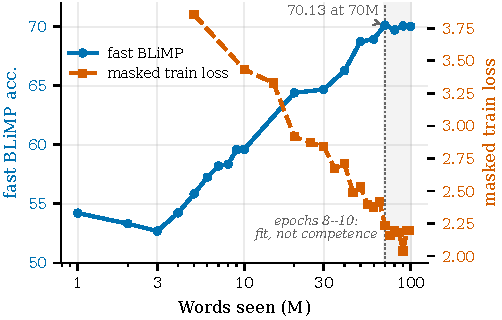
\includegraphics[width=\columnwidth]{figures/fig_saturation}
  \caption{\textbf{The budget saturates early.} Fast BLiMP accuracy (left axis)
  reaches \rBlimpPeak{} by \rPeakCkpt{} words seen and is flat from there,
  while the
  masked training loss (right axis) keeps falling to the end of training. The
  final epochs lower the loss without improving competence.}
  \label{fig:saturation}
\end{figure}


\subsection{Reallocating the Wasted Budget with \MPO{}}
\label{sec:method}
\begin{figure*}[t]
  \centering

  % Shrink the entire TikZ diagram to 80% of its original size
  \scalebox{0.85}{%
  \begin{tikzpicture}[
    font=\small,
    box/.style={
      rounded corners=2pt,
      draw,
      thick,
      minimum height=8mm,
      inner sep=3pt,
      align=center
    },
    lab/.style={font=\footnotesize\itshape, text=black!60},
    >=stealth,
  ]

    % ---------------- top band: pretraining timeline ----------------
    \draw[->, thick, black!55] (0,0) -- (14.0,0)
      node[right, black!70]{words seen};

    \foreach \x/\t in {0/0,3.5/50M,4.9/70M,9/100M}
      \draw[black!45] (\x,0.06)--(\x,-0.06)
        node[below,font=\scriptsize,black!60]{\t};

    \draw[very thick,MYblue]
      plot[smooth] coordinates
      {(0,0.4) (1.2,1.0) (2.4,1.7) (3.5,2.15) (4.2,2.35) (4.9,2.45)};

    \draw[very thick,MYblue,dash pattern=on 2pt off 2pt]
      (4.9,2.45)--(9,2.45);

    \node[MYblue,font=\footnotesize\bfseries]
      at (2.0,2.75) {MLE pretraining};

    \node[lab]
      at (6.95,2.78)
      {epochs 8--10: fit, not competence (wasted)};

    \fill[black!70] (4.9,2.45) circle (1.4pt);

    \node[align=center,font=\scriptsize,black!70]
      at (4.9,1.75)
      {saturation ckpt\\(\textbf{7 ep, 70M})};

    \node[font=\footnotesize\bfseries,MYgreen!55!black]
      at (11.7,2.45)
      {71.3M $\ll$ 100M budget};

    % ---------------- fork ----------------
    \draw[->,very thick,MYorange]
      (4.9,1.35)
      .. controls (4.9,0.4) and (4.6,-0.4) ..
      (4.6,-0.95);

    % ---------------- MPO contents ----------------

    \node[
      box,
      fill=MYblue!10,
      draw=MYblue!60,
      font=\scriptsize,
      minimum width=34mm
    ] (pos) at (3.05,-2.15)
      {$x^{+}$: real corpus sentence};

    \node[
      box,
      fill=MYred!8,
      draw=MYred!55,
      font=\scriptsize,
      minimum width=34mm,
      minimum height=10mm
    ] (neg) at (3.05,-3.35)
      {$x^{-}$: length-preserving\\corruption of $x^{+}$};

    \node[
      box,
      fill=MYgreen!10,
      draw=MYgreen!60,
      font=\scriptsize,
      minimum width=26mm
    ] (pol) at (7.3,-2.15)
      {policy $\pi_\theta$\\{\scriptsize init $=$ ckpt}};

    \node[
      box,
      fill=black!5,
      draw=black!45,
      font=\scriptsize,
      minimum width=26mm
    ] (ref) at (7.3,-3.35)
      {frozen $\pi_{\text{ref}}$\\{\scriptsize KL anchor}};

    \draw[->,MYblue!70] (pos)--(pol);
    \draw[->,MYred!70] (neg)--(pol);
    \draw[->,black!40]
      (pos.east)--++(0.35,0)|-(ref.west);

    \node[
      box,
      fill=none,
      draw=MYorange!50,
      densely dashed,
      font=\scriptsize,
      minimum width=32mm
    ] (obj) at (11.2,-2.15)
      {prefer $x^{+}\!\succ\!x^{-}$\\{\scriptsize (DPO, Eq.~\ref{eq:dpo})}};

    \node[
      lab,
      align=center,
      text width=32mm
    ] (retain) at (11.2,-3.35)
      {\;+\; retain-MLE mix\\{\scriptsize preserve competence}};

    \draw[->,thick,MYgreen!60!black]
      (pol)--(obj);

    % ---------------- background yellow box ----------------
    \begin{pgfonlayer}{background}
      \node[
        rounded corners=3pt,
        draw=MYorange!70,
        fill=MYorange!7,
        thick,
        inner xsep=8mm,
        inner ysep=8mm,
        fit=(pos)(neg)(pol)(ref)(obj)(retain)
      ] (dpo) {};
    \end{pgfonlayer}

    % ---------------- title ----------------
    \node[
      anchor=north,
      font=\footnotesize\bfseries,
      text=MYorange!80!black
    ] at ([yshift=-2mm]dpo.north)
    {\MPO{} post-training (+1.3M word-touches $\to$ 71.3M total)};

  \end{tikzpicture}%
  } % end scalebox

  \caption{\textbf{Reallocating the wasted budget.} MLE pretraining saturates at
  the \textbf{7-epoch / 70M-word} checkpoint (dashed tail $=$ the wasted epochs of
  Fig.~\ref{fig:saturation}). We fork there into \textbf{\MPO{}}: the model is
  taught to prefer a real corpus sentence $x^{+}$ over a length-preserving
  corruption $x^{-}$ of itself, KL-anchored to a frozen copy of the same
  checkpoint and mixed with a retain-MLE term (\S\ref{sec:method}). Total
  exposure is 71.3M words, well under the 100M budget, and fewer than the
  fully-trained baseline.}

  \label{fig:method}
\end{figure*}


The diagnosis licenses three design principles. The first is \emph{timing}:
refinement signal should arrive only after acquisition has saturated, where
it no longer competes with the language-modeling gradient for capacity
(\S\ref{sec:search} tests the necessity of this). The second is
\emph{preservation}: additions must be bounded in how far they can move the
model, because $\mathcal{F}$ is what a strong new gradient destroys first.
The third is \emph{alignment}: the signal should share the evaluation's
functional form, which for BLiMP, its supplement, EWoK, and entity tracking
is a relative-likelihood comparison between minimally different strings.
\MPOlong{} (\MPO{}) instantiates all three (Figure~\ref{fig:method}).

Preference data comes from the corpus itself: no teacher, no reward model,
no annotator, and no text beyond the ten million words already budgeted. A
real sentence $x^{+}$ becomes $x^{-} = T(x^{+})$ with $T$ drawn uniformly
from four edit operators, each length-preserving ($|T(x)| = |x|$): an
adjacent-token swap, a distant-token swap, a function-word substitution, and a
random content-token replacement. On \emph{the cat sat on the mat} these
produce, respectively, \emph{the cat on sat the mat}, \emph{the mat sat on
the cat}, \emph{the cat sat of the mat}, and \emph{the cat lamp on the
mat}. The four target complementary structure,
from local word order to exactly the long-range configuration $\mathcal{F}$
tests: the adjacent swap probes local agreement, the distant swap and the
function-word substitution probe the long-range dependencies of
$\mathcal{F}$, and the random replacement supplies an easily rejected
contrast that anchors the low end of the difficulty range.
Appendix~\ref{sec:app-ops} ablates each operator alone and confirms the
complementarity. The phase touches under $3\%$ of the \rSentBank{} corpus sentence
units, derives nothing from any evaluation resource, and introduces no new
word types; the corruptions are input noise of the same kind the masked
objective has injected since the first step of pretraining, which already
replaces sampled tokens at random.

Length matching makes the comparison fair by construction. Every edit
operates in place on the tokenized sentence, so $x^{+}$ and $x^{-}$ contain
the same number of tokens and their summed causal log-likelihoods,
\begin{equation}
\label{eq:seqll}
\ell_\theta(x) \;=\; \textstyle\sum_{t}\, \log \pi_\theta\!\big(x_t \mid x_{<t}\big),
\end{equation}
are directly comparable with no normalization to tune, mirroring the
minimal-pair design of BLiMP itself. (The suite scores the hybrid through
a masked backend, \S\ref{sec:submission}; what the phase shares with the
evaluation is this comparison structure, not the scoring function.) Given
pairs, we optimize the DPO objective \citep[cf.][]{rafailov2023dpo}:
\begin{equation}
\label{eq:dpo}
\resizebox{0.89\columnwidth}{!}{$
\mathcal{L}_{\text{\MPO{}}}(\theta) = -\,\mathbb{E}\Big[\log \sigma\Big(\beta\big[\Delta_\theta(x^{+}) - \Delta_\theta(x^{-})\big]\Big)\Big],
$}
\end{equation}
with $\Delta_\theta(x) = \ell_\theta(x) - \ell_{\text{ref}}(x)$. The
reference is a frozen copy of the checkpoint the policy starts from, and in
the reward-maximization problem that Eq.~\ref{eq:dpo} solves implicitly,
$\beta$ is the coefficient on $\mathrm{KL}(\pi_\theta \,\|\, \pi_{\text{ref}})$
\citep{rafailov2023dpo}. Preservation therefore enters the objective
directly rather than being assumed: likelihoods may reorder so that real
sentences win, but drift
from existing competence is penalized at rate $\beta=\rBeta$. This
property is what selects DPO among pairwise objectives: an anchor-free
ranking loss would leave preservation to the learning rate alone, and the
nearest anchor-free relative in this paper, the contrastive arm of
\S\ref{sec:search}, is the study's clearest failure. That arm also
supplies the closest control: the same four corruptions, injected during
acquisition without an anchor and under a loss free to reshape the model,
cost seven BLiMP points. The corruption data was never the problem; what
changed between failure and success is when the signal arrives and how
tightly it is held. Because preference
optimization alone slowly erodes general language-modeling quality, a failure
mode documented in the RLHF literature, the step-$t$ loss retains the
pretraining signal,
\begin{equation}
\label{eq:phase}
\resizebox{0.89\columnwidth}{!}{$
\mathcal{L}_{\text{phase}}(\theta) = \mathcal{L}_{\text{\MPO{}}}(\theta) + m_t\,\mathcal{L}(\theta),
\quad m_t \sim \mathrm{Bernoulli}(0.5),
$}
\end{equation}
one ordinary hybrid micro-batch (Eq.~\ref{eq:hybrid}, post-anneal
masking rate) at unit weight.

The timing principle fixes the starting point. Policy and reference
initialize from the 70M-word saturation checkpoint, not the fully-trained
model; running the identical phase from the 99M-word checkpoint reaches the
same BLiMP (\S\ref{sec:results-ablations}) at 29M additional words of
budget, direct evidence that epochs eight through ten contributed nothing
the method requires. Starting earlier does not substitute for acquisition:
from the
pre-saturation 30M checkpoint the same phase leaves fast BLiMP at
\rInitThirtyB{}, barely above that checkpoint's own \rThirtyBaseB{}. The
phase refines competence; it does not create it. Total exposure is 70M plus roughly \rDpoPhaseWords{} phase
word-touches, counted conservatively: every token of both members of every
pair and of the retained hybrid batches is charged against the budget, for
\rDpoWords{} in all, well inside the 100M cap a 10-epoch run would exhaust
(Appendix~\ref{sec:app-budget} itemizes the accounting).

The configuration is deliberately conservative: \rDpoSteps{} AdamW steps at
learning rate $\rDpoLR$, \rDpoPairs{} pairs per step, cosine decay,
clipping at $1.0$, about \rDpoMinutes{} minutes on the same laptop (roughly
$3\%$ of the pretraining wall-clock), checkpoints every 250 steps.
\S\ref{sec:results-ablations} shows a plateau across those checkpoints
rather than a single favorable snapshot, and shows that a stronger
preference objective improves its own training metrics while degrading the
evaluation; the restraint is functional rather than stylistic.
